\label{Figure Model Variation}
\begin{figure}[H]
    \centering
    \begin{subfigure}{0.17\textwidth}
        \centering
        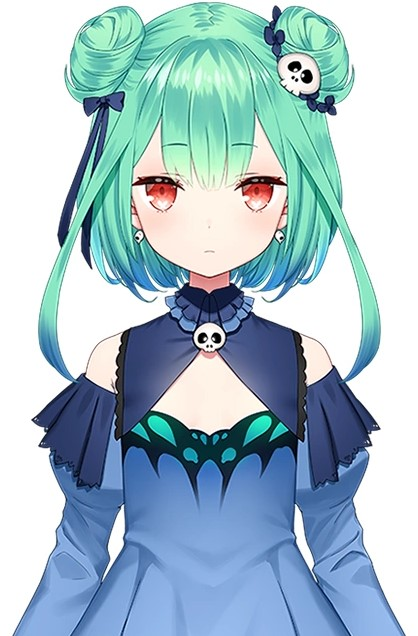
\includegraphics[width=\textwidth]{images/variation/ru1.jpg}
        \caption{Original\cite{rushiaoriginal}}
        \label{fig:ru1}
    \end{subfigure}
    \hfill
    \begin{subfigure}{0.17\textwidth}
        \centering
        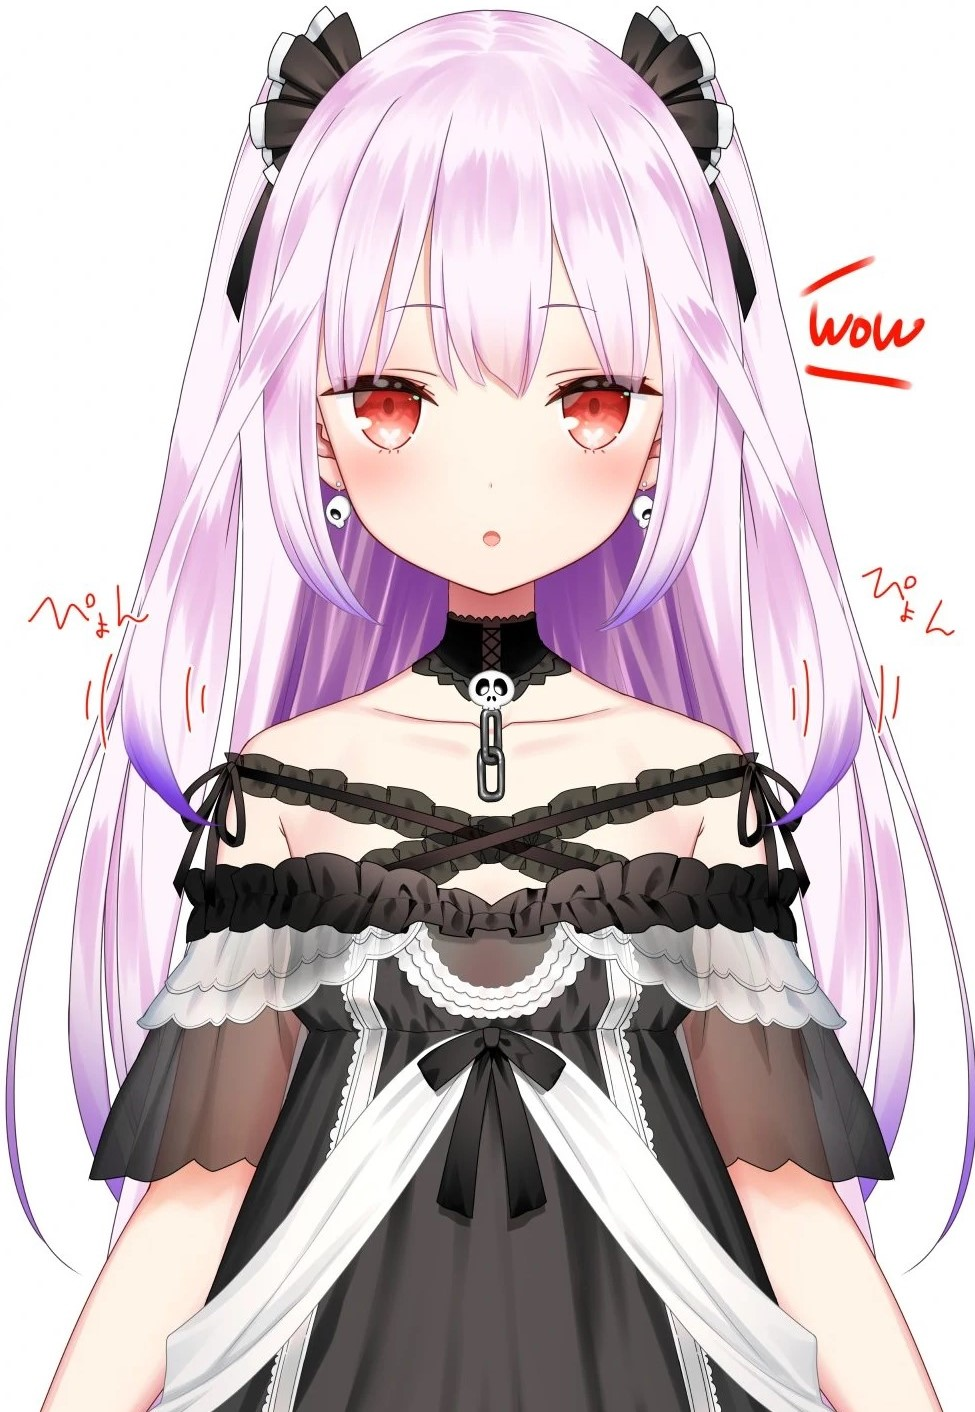
\includegraphics[width=\textwidth]{images/variation/ru2.jpg}
        \caption{Alternative\cite{rushiaalternative}}
        \label{fig:ru2}
    \end{subfigure}
    % \begin{flushleft}
    %     (a) Original outfit\\
    %     (b) Alternative outfit
    % \end{flushleft}
    \caption{Model variation}
    \label{fig:modelvariation}
\end{figure}